\section*{Question 2}
We now wish to introduce \textit{less than or equals} to the program. This is done, inspired by one of the productions from the \texttt{base\_bool\_expr}: BBE $\rightarrow$ AE '=' AE. Instead of just '=' it must recognice '$<$=' also. This needs to be added to the abstract syntax tree (written in java) by creating a class similar to the \texttt{EqualsExpr} class, called \texttt{LessOrEqualsExpr}. The main content of this class is seen in the code snippet below:

\begin{lstlisting}
private ArithExpr expr1, expr2;
public LessOrEqualsExpr(ArithExpr expr1, ArithExpr expr2) {
	this.expr1 = expr1;
	this.expr2 = expr2;
}

@Override
public boolean evaluate(Environment env) throws VariableNotDefinedException {
	return expr1.evaluate(env) <= expr2.evaluate(env);
}
\end{lstlisting}

This class simply takes two parameters in the constructor: the expressions to be checked, and the evaluation uses java's build in \textit{less than or equals} operation. 


Similarly, we now wish to introduce \textit{not equals} to the program. This is done easily, using the supplied classes \texttt{NotExpr} and \texttt{EqualsExpr}, meaning that no new abstract syntax needs to be introduced. The complete \texttt{base\_bool\_expr} rule in the while language, is seen in the code snippet below:

\begin{lstlisting}
base_bool_expr returns [BoolExpr value]
  : 'true'    { $value = new BoolValueExpr(true); }
  | 'false'   { $value = new BoolValueExpr(false); }

  //NEW
  | e1=arith_expr '<=' e2=arith_expr  { $value = new LessOrEqualsExpr(e1, e2); }
  
  //NEW
  | e1=arith_expr '!=' e2=arith_expr  { $value = new NotExpr(new EqualsExpr(e1,e2)); }

  | e1=arith_expr '=' e2=arith_expr   { $value = new EqualsExpr(e1,e2); }
;
\end{lstlisting}

As seen the not equals uses the NotExpr and the EqualsExpr syntax nested. The order here is not relevant.


The two new rules can be seen in use, in figure \ref{fig:Q2ex}.

\begin{figure}[H]
    \centering
    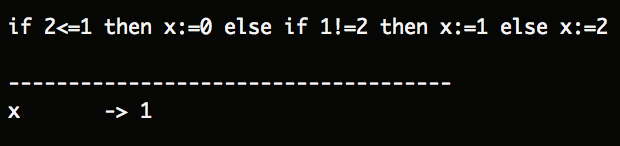
\includegraphics[width=0.5\textwidth]{fig/Q2example}
    \caption{Example of '$<$=' and '!=' with correct answer of x = 1. Above the horizontal lines describe the program input, and below the output.}
    \label{fig:Q2ex}
\end{figure}